\section{Analysis: Comparison with Predictive Coding Framework and Gap-Junction Coupling}


Here we compare the self-coupled model with the predictive coding framework (PCF) as defined in Boerlin \& Deneve, 2013. We demonstrate that an assumption in this model leads to a network estimate whose accuracy indefinitely diverges with time. The correction of this assumption leads to an intermittent model featuring membrane voltage coupling we loosely term gap-junction coupling. We show that the gap-junction model rectifies network estimation error introduced by the PCF. We then show that the corrected gap-junction model and the self-coupled mode produce identical results.

\begin{enumerate}

\item \textbf{\textit{The Predictive Coding Framework (PCF):}} The PCF synthesizes a spiking neural network that implements a given dynamical system. It is briefly derived as follows:\\
\\
Assume we are given in dimensionless form
\begin{itemize}
    \item A Linear Dynamical System  $\dot{x}(\xi) = A x(\xi) + B c(\xi)$,  $x \in \mathbf{R}^d$
    
    \item A Decoder Matrix $D \in \mathbf{R}^{d\hspace{1mm} x \hspace{1mm}N}$ specifying The tuning curve of N neurons in d-dimensional space. \\
\end{itemize}
Let $o(t) \in \mathbf{R}^{N}$ describe the spike trains whose $j^{th}$ component is given by
\begin{align*}
	o_j(t) \overset{\Delta}{=} \sum_{k=0}^{\infty} \delta(t - t_j^k),
\end{align*} 
where $t_j^k$ is the time of the $k^{th}$ spike of neuron $j$. 
Define the time-varying firing rate of the neurons by 
\begin{align*}
	\frac{d r}{d t}(t) \overset{\Delta}{=} - \tau_s^{-1} r(t) + \tau_s^{-1} o(t),
\end{align*}
where $\tau_s{-1}$ is the decay rate of $r(t)$ given by the inverse synaptic time constant $\tau_s$. For consistency across models, we transform the preceding two equations to dimensionless time via $\xi = \frac{t}{\tau_s} \implies  \tau_s \, d \xi = dt$. This gives
\begin{align}
	\label{eq:analysis:comparison_sc_vs_pcf_vs_gj:pcf_o_def}
	o_j(\xi) \overset{\Delta}{=} \sum_{k=0}^{\infty} \delta(\xi - \xi_j^k),
\end{align}
where $\xi_j^k$ is the $k^{th}$ spike of neuron $j$ in dimensionless time, and
\begin{align*}
	\frac{d r}{d t}(t) &= - \tau_s^{-1} r(t) + \tau_s^{-1}o(t),
	\\
	\\
	\implies
	\frac{d r}{\tau_s \, d \xi}(\xi) &= - \tau_s^{-1} r(\xi) + \tau_s^{-1} o(\xi),
	\\
	\\
	\implies
	\frac{dr}{d\xi}(\xi) &= - r(\xi) + o(\xi).
\end{align*}    
Letting $\dot{\left[ \hspace{5mm} \right]}$ denote differentiation w.r.t. dimensionless time $\xi$, we arrive at 
\begin{align}
\label{eq:analysis:comparison_sc_vs_pcf_vs_gj:pcf_r_def}
\dot{r}(\xi) \overset{\Delta}{=} - r(\xi) + o(\xi). 
\end{align}

The network estimate is defined as 
\begin{align}
\label{eq:analysis:comparison_sc_vs_pcf_vs_gj:pcf_xhat_def}
\hat{x}(\xi) \overset{\Delta}{=} D r(\xi),
\end{align}
which gives rise to the network estimation error
\begin{align}
\label{eq:analysis:comparison_sc_vs_pcf_vs_gj:pcf_error_def}
e(\xi) \overset{\Delta}{=} x(\xi) - \hat{x}(\xi).
\end{align}

The network chooses spike times $\xi_j^k$ to greedily optimize the objective function
\begin{align*}
\mathcal{L}(\xi) = ||x(\xi + d\xi) - \hat{x}(\xi + d\xi)||^2.
\end{align*}
The PCF uses regularization on the rate $r(\xi)$ for the sake of biological plausibility. At present we ignore this regularization and note that they can only increase the network estimation error $e$, the sole network objective.
Using an identical approach to the derivation of the self-coupled network in section (\ref{section:derivation:basic_model}), we arrive at 
\begin{align*}
d_j^T 
\left(
	x - \hat{x}
\right)
&= 
\frac{d_j^T d_j}{2}
\end{align*}
where $d_j$ is the $j^{th}$ column of $D$. We define membrane voltage to get the spiking condition:
\begin{align}
\label{eq:analysis:comparison_sc_vs_pcf_vs_gj:pcf_voltage_def}
v_j &\overset{\Delta}{=} d_j^T (x - \hat{x}) 
\notag
\\
\\
\notag
\implies
d_j^T e &= v_{th}, 
\end{align}

where $v^{th} = \frac{d_j^T d_j}{2}$.

Deriving the dynamics, the preceding equation defines voltage, which in matrix form is given by
\begin{align*}
V &= D^T 
\left(
	x - \hat{x}
\right)
%
\\
\\
%
\implies
\dot{V}
&= 
D^T \dot{x} - D^T \dot{\hat{x}}
&
\\
\\
%
&= D^T 
\left(
	A x + B c
\right)
 - D^T 
 \left(
 D \dot{r}
 \right)
 %
 \\
 \\
 %
 &= 
 D^T A x
 + D^T B c
 - D^T D
\left(
	-r + o 
\right) 
 .
\end{align*}
The PCF makes the assumption that when the network performs correctly, $x = \hat{x}$. We later quantify the estimation error introduced by this assumption and correct it to form the gap-junction model. For now make the assumed substitution $x = \hat{x} = Dr$. 

\begin{align*}
\dot{V} &= D^T A \left(D r\right) + D^T B c + D^T D r - D^T D o
%
\\
\\
%
&= 
D^T
\left(
	A + I 
\right)
 D r
+
D^T B c 
- D^T D o. 
\end{align*}

The model is finalized by the addition of a voltage leakage term to ensure stability, giving the final dynamics equation

\begin{align}
\label{eq:analysis:comparison_sc_vs_pcf_vs_gj:pcf_voltage_dynamics}
\dot{V} = -v
+ D^T 
\left(
A + I
\right)
D r
+ 
D^T B c
- D^T D o.
\end{align}

Equation (\ref{eq:analysis:comparison_sc_vs_pcf_vs_gj:pcf_voltage_dynamics}) scales the spike train $o_j$ by $d_j^T d_j$. Thus the spiking behavior is described by
\begin{align}
\label{eq:analysis:comparison_sc_vs_pcf_vs_gj:pcf_spiking_behavior}
    &v_{th} = \frac{ d_j^T d_j }{2} \notag \\
    \notag \\
    &\text{if  } v_j > v^{th}_j,\notag \\
    \\
    &\text{then  } v_j^{'} = v_j - d_j^T d_j \int \delta(\tau)  \, d\tau ,\notag \\
    \notag \\ 
    &\text{and  } r_j^{'} = r_j + \int \delta(\tau)  \, d\tau \notag.
\end{align}
Equations (\ref{eq:analysis:comparison_sc_vs_pcf_vs_gj:pcf_voltage_dynamics}) and (\ref{eq:analysis:comparison_sc_vs_pcf_vs_gj:pcf_spiking_behavior}) specify the PCF model we compare against. Figure (\ref{fig:analysis:comparison_sc_vs_pcf_vs_gj:pcf_network_decode_demo}) shows simulations of the PCF model with the following parameters:

\begin{align}
\label{eq:analysis:comparison_sc_vs_pcf_vs_gj:pcf_demo_sim_params}
A &= -\begin{bmatrix}  
1 & 0 \\
0 & 1
\end{bmatrix},\notag \\
\notag \\
B &= \begin{bmatrix}  
1 & 0 \\
0 & 1
\end{bmatrix}, \notag \\
\notag \\
c(\xi) &= 10 \begin{bmatrix} 
cos(\frac{\pi}{2} \xi)\\
sin(\frac{\pi}{2} \xi)
\end{bmatrix} + 8 \\
\notag \\
D_{\text{ij}} &\sim  \mathcal{N} (0, 1) \text{ Columns Normalized to Unit Length} \notag \\
\notag \\
d\xi &= 10^{-5}, \notag \\
\notag \\
N &= 32,\notag \\
\notag \\
x(0) &= \begin{bmatrix} \frac{1}{2} & \frac{1}{2} \end{bmatrix}.\notag 
\end{align}\\



% Simulate PCF model here, display error vs time for long-term evolution, highlight this divergence
\begin{figure}
\centering
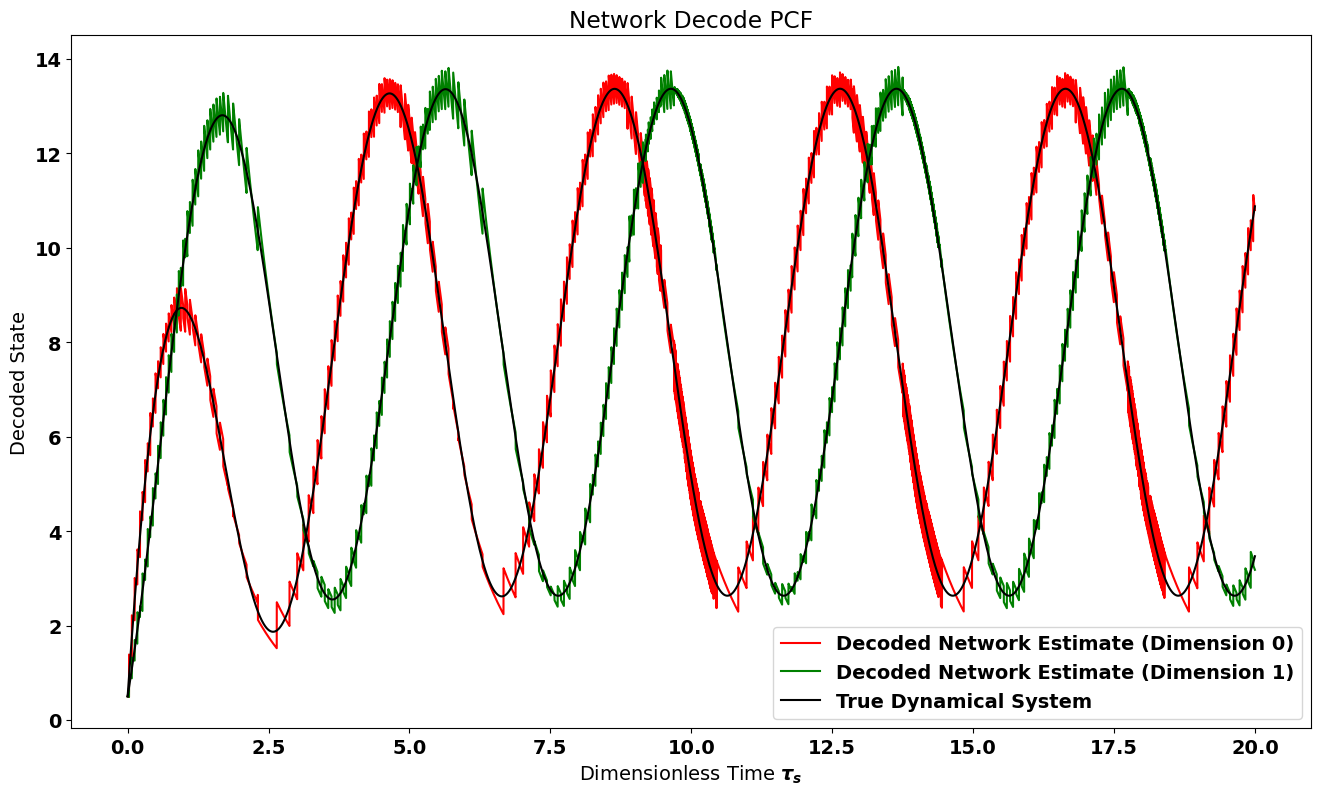
\includegraphics[width=\linewidth]{figures/network_decode_PCF.png}
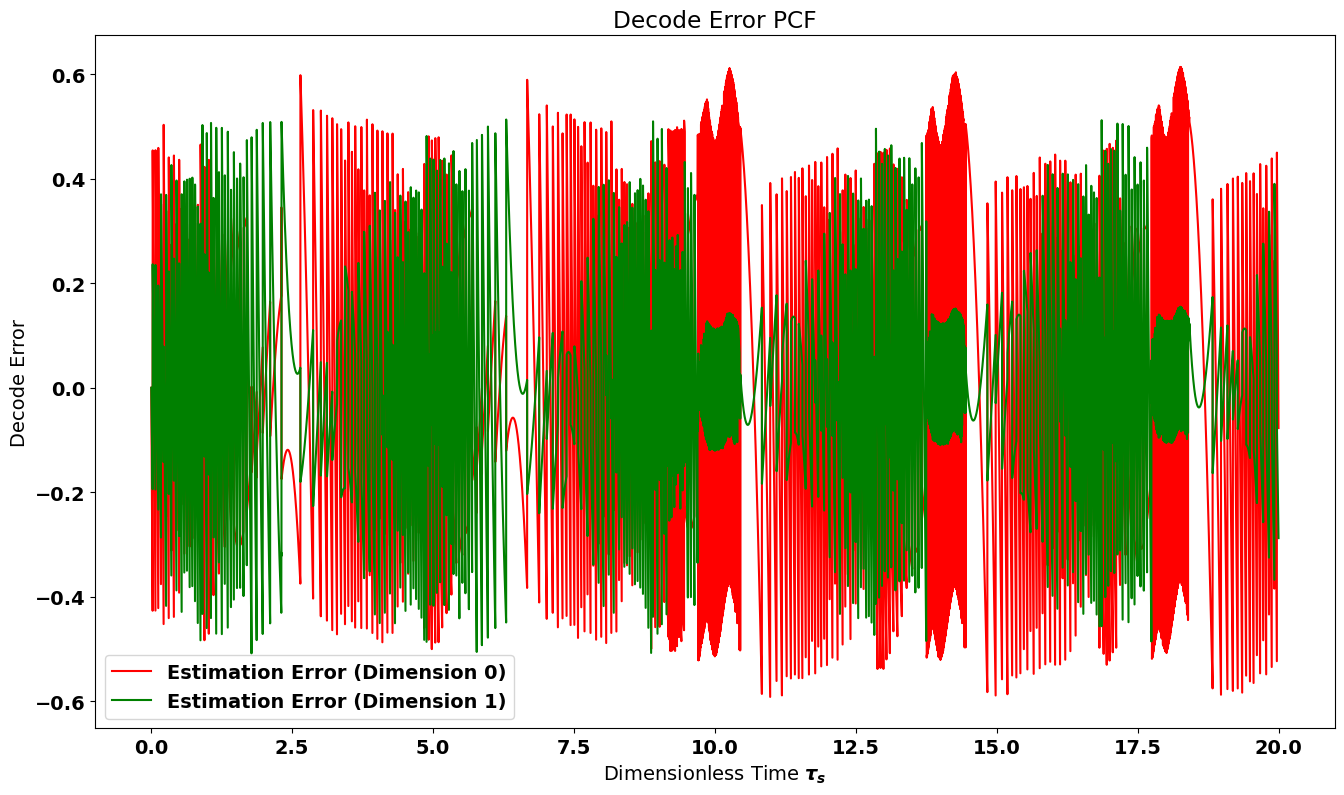
\includegraphics[width=\linewidth]{figures/decode_error_PCF.png}
\caption{Simulation of PCF model given by equations (\ref{eq:analysis:comparison_sc_vs_pcf_vs_gj:pcf_spiking_behavior}) and (\ref{eq:analysis:comparison_sc_vs_pcf_vs_gj:pcf_voltage_dynamics}). \textbf{\textit{Top:}} Network estimate given by equation (\ref{eq:analysis:comparison_sc_vs_pcf_vs_gj:pcf_xhat_def}). \textbf{\textit{Bottom:}} Estimation Error for PCF network from equation (\ref{eq:analysis:comparison_sc_vs_pcf_vs_gj:pcf_error_def}). The simulation parameters are given in equation (\ref{eq:analysis:comparison_sc_vs_pcf_vs_gj:pcf_demo_sim_params}). The numerical implementation is identical to that in section (\ref{section:derivation:basic_model}). A Pad\'e approximation is used to compute a matrix exponential, then used to integrate the continuous terms of the differential equations. The spikes are handled separately at each time step by manually changing the values of neurons above threshold.  For reasons of numerical stability, only one spike per time-step is allowed in the PCF model.  
}
\label{fig:analysis:comparison_sc_vs_pcf_vs_gj:pcf_network_decode_demo}
\end{figure}

\clearpage

\item 
\textbf{\textit{The Gap-Junction Correction:}} Here we correct the assumption that $\hat{x} = x$ made in the PCF model. We restart the previous derivation from this point and derive more a accurate form of equation (\ref{eq:analysis:comparison_sc_vs_pcf_vs_gj:pcf_voltage_dynamics}) termed the gap-junction model.\\
The derivation is identical as the PCF until we derive the voltage dynamics.

\begin{align*}
\dot{V} &= 
D^T A x
+
D^T B c
+ D^T D r
- D^T D o.
\end{align*}
Instead of assuming $x = \hat{x}$, we apply the definition of voltage, equation (\ref{eq:analysis:comparison_sc_vs_pcf_vs_gj:pcf_voltage_def}) in matrix form.
\begin{align*}
v_j &= d_j^T e 
%
\\
\\
%
\implies 
V &= D^T e
%
\\
\\
%
&= 
D^T 
\left(
x - \hat{x}
\right)
%
\\
\\
%
\implies
x 
&=
D^{T \dagger} V  + \hat{x}
%
\\
\\
%
&=
D^{T \dagger} V + D r,
\end{align*}
where $D^{T \dagger}$ is the left Moore-Penrose pseudo-inverse of $D^T$.
Substitute this for $x$ in $\dot{V}$ above to get
\begin{align}
\label{eq:analysis:comparison_sc_vs_pcf_vs_gj:gj_voltage_dynamics}
\dot{V} &= 
D^T A
\left(
	D^{T \dagger} V + D r
\right)
+ D^T D r
+
D^T B c
- D^T D o 
\notag
% 
\\ \notag
\\ 
%
\implies
\dot{V}
&= 
D^T A
D^{T \dagger} V 
+
D^T
\left(
	A + I 
\right)
D r
+ 
D^T B c
- D^T D o.
\end{align}

Equation (\ref{eq:analysis:comparison_sc_vs_pcf_vs_gj:gj_voltage_dynamics}) in conjunction with an identical spiking rule from PCF, equation (\ref{eq:analysis:comparison_sc_vs_pcf_vs_gj:pcf_spiking_behavior}) specifies the gap-junction model. It is simulated in figure (\ref{fig:analysis:comparison_sc_vs_pcf_vs_gj:gj_network_decode_demo}). While the two simulations are similar, there are noticeable differences in their behavior e.g. $\tau_s \simeq 10, \, 13$. 

\begin{figure}
\centering
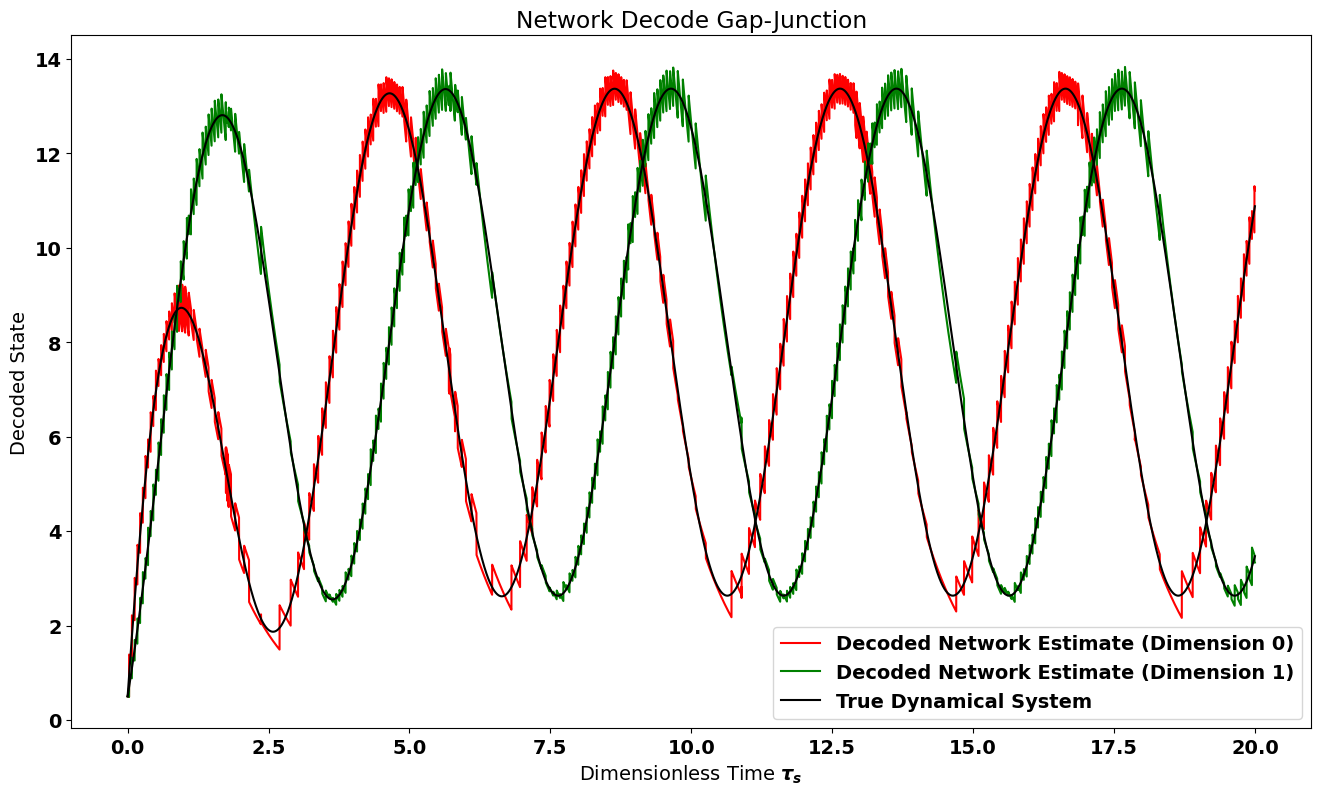
\includegraphics[width=\linewidth]{figures/network_decode_Gap-Junction.png}
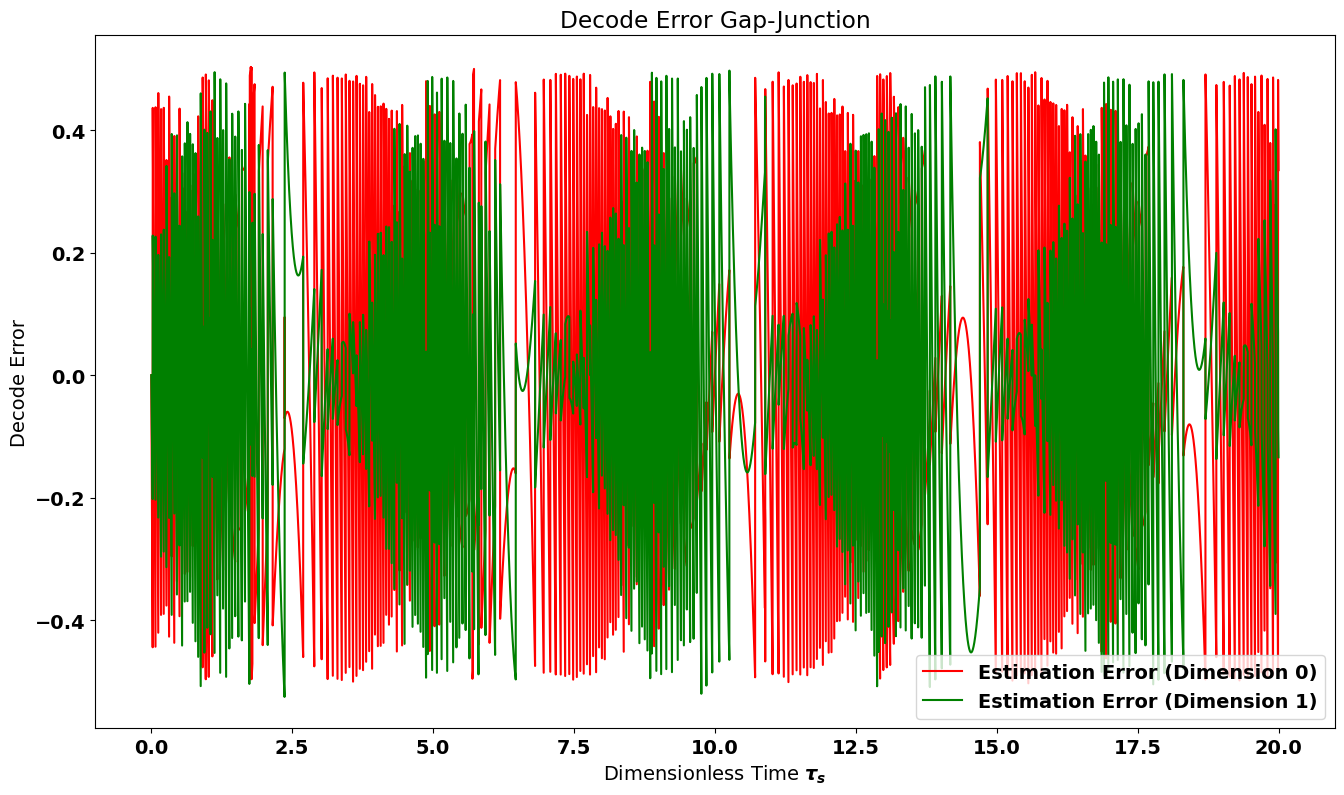
\includegraphics[width=\linewidth]{figures/decode_error_Gap-Junction.png}
\caption{Simulation of the Gap-Junction model given by equations (\ref{eq:analysis:comparison_sc_vs_pcf_vs_gj:pcf_spiking_behavior}) and (\ref{eq:analysis:comparison_sc_vs_pcf_vs_gj:gj_voltage_dynamics}). \textbf{\textit{Top:}} Network estimate given by equation (\ref{eq:analysis:comparison_sc_vs_pcf_vs_gj:pcf_xhat_def}). \textbf{\textit{Bottom:}} Estimation Error for the Gap-Junction network from equation (\ref{eq:analysis:comparison_sc_vs_pcf_vs_gj:pcf_error_def}). The simulation parameters are the same as the previous figure. As with the PCF model, the network is only numerically stable if spikes are restricted to one per time step. 
}
\label{fig:analysis:comparison_sc_vs_pcf_vs_gj:gj_network_decode_demo}
\end{figure}


%The PCF and gap-junction models differ only in their voltage dynamics equations, (\ref{eq:analysis:comparison_sc_vs_pcf_vs_gj:pcf_voltage_dynamics}) and (\ref{eq:analysis:comparison_sc_vs_pcf_vs_gj:gj_voltage_dynamics}) respectively. Suppose we use both models to simulate a target dynamical system. Denote the estimate of the PCF network as $\hat{x}_{pcf}$, and the estimate of the gap-junction network as $\hat{x}_{gj}$. We wish to derive the difference between these estimates denoted by $\chi$. 
%\begin{align}
%	\label{eq:analysis:comparison_sc_vs_pcf_vs_gj:pcf_vs_gj_estimation_error_def}
%	\chi \hspace{2mm} \overset{\Delta}{=} \hspace{2mm} \hat{x}_{pcf} - \hat{x}_{gj}.
%\end{align}
%
%To compute $\chi$, invert our voltage definition equation (\ref{eq:analysis:comparison_sc_vs_pcf_vs_gj:pcf_voltage_def}) in matrix form to get
%\begin{align*}
%V
%&= 
%D^T
%\left(
%	x - \hat{x}
%\right)
%%
%\\
%\\
%%
%\implies 
%\hat{x}
%&= 
%x - D^{T \dagger} V
%%
%\\
%\\
%%
%\implies
%\hat{x}_{pcf} - \hat{x}_{gj}
%&= 
%\chi
%%
%\\
%\\
%%
%&= 
%D^{T \dagger} 
%\left(
%	V_{gj} - V_{pcf}
%\right)
%%
%\\
%\\
%%
%\implies 
%\dot{\chi} 
%&= 
%D^{T \dagger} 
%\left(
%	\dot{V}_{gj} -
%	\dot{V}_{pcf}
%\right). 
%\end{align*}
%
%
%Subtract the right hand sides of equation (\ref{eq:analysis:comparison_sc_vs_pcf_vs_gj:pcf_voltage_dynamics})from (\ref{eq:analysis:comparison_sc_vs_pcf_vs_gj:gj_voltage_dynamics}) to get
%
%\begin{align*}
%\dot{V}_{gj} - \dot{V}_{pcf} 
%&=
%D^T A
%D^{T \dagger} V_{gj} + V_{pcf}
%%
%\\
%\\
%%
%\implies
%\dot{\chi}
%&=
%A D^{T \dagger} V_{gj}
%+ 
%D^{T \dagger} V_{pcf}
%%
%\\
%\\
%%
%&= 
%A D^{T \dagger} V_{gj}
%+ 
%D^{T \dagger} V_{pcf}
%-
%A D^{T \dagger} V_{pcf}
%+
%A D^{T \dagger} V_{pcf}
%-
%D^{T \dagger} V_{gj}
%+
%D^{T \dagger} V_{gj}
%%
%\\
%\\
%%
%&= 
%A D^{T \dagger} 
%\left(
%	V_{gj} - V_{pcf}
%\right)
%+ A D^{T \dagger}  V_{pcf}
%+ 
%D^{T \dagger} 
%\left(
%	V_{pcf} - V_{gj}
%\right)
%+
%D^{T \dagger} V_{gj}
%%
%\\
%\\
%%
%&=
%\left(
%	A - I
%\right)
%\chi
%+ 
%A D^{T \dagger}  V_{pcf}
%+
%D^{T \dagger} V_{gj}
%\end{align*}

\clearpage

\item \textbf{\textit{Spike Rate Laws:}} Here we explicitly solve the for the steady state behavior of the PCF and gap-junction models in response to a constant stimulus. We compute their per-spike RMSE and compare each with the self-coupled network model. 

Let all 3 models have the same parameters as given by equation (\ref{eq:analysis:comparison_sc_vs_pcf_vs_gj:pcf_demo_sim_params}) with the exception that 

\begin{align*}
	c(\xi) &= c = 
	\begin{bmatrix}
		1 \\ 0	
	\end{bmatrix}, 
\end{align*}
and
$x(0) = \begin{bmatrix} \frac{1}{2} & 0 \end{bmatrix}$. From equation (\ref{eq:analysis:comparison_sc_vs_pcf_vs_gj:pcf_voltage_dynamics}), the PCF dynamics become
\begin{align*}
	\dot{V}_{pcf}
	&=
	- V_{pcf}
	+
	D^T 
	\left(
		-I + I
	\right)
	D^T r
	+
	D^T 
	\begin{bmatrix}
		1 \\ 0
	\end{bmatrix}
	-
	D^T D o
	%
	\\
	\\
	%
	&= 
	-V_{pcf}
	+ 
	D^T 
	\begin{bmatrix}
		1 \\ 0
	\end{bmatrix}
	-
	D^T D o.
\end{align*}
All voltages are initially 0. From equation (\ref{eq:analysis:comparison_sc_vs_pcf_vs_gj:pcf_spiking_behavior}) the thresholds are identically $\frac{1}{2}$. Until the first spike, neuron $j$'s voltage integrates the quantity $d_j^T 	\begin{bmatrix}	1 \\ 0	\end{bmatrix}$. Denote the neuron $j$ whose tuning curve $d_j$ is closest in angle to $c$ by 

\begin{align*}
	j_{max} \overset{\Delta}{=}
	 \underset{
	 	i \in 
	 	\left[
	 		1, \ldots, N
	 	\right]
	 }
	 {argmax}
	 \hspace{4mm}
	 	d_j^T c.
\end{align*}
Neuron $j_{max}$ will receive the highest driving force and will therefore reach its threshold  before any other neuron. It will then be reset by $1$ to $- \frac{1}{2}$. Each other neuron $k$ will also be reset (decremented) by $d_k^T d_{j_{max}}$, proportional to their angle relative to both neuron $j_{max}$ and the driving strength $c$. This sequence will repeat periodically so that only neuron $j_{max}$ fires at a constant rate. 

We write the PCF network as the one-dimensional equation

\begin{align*}
	v_{pcf} &= 
	- v_{pcf}
	+ d_{j_{max}}^T c 
	- o_{j_{max}}.
\end{align*}

This is a form of the leaky integrate-and-fire (LIF) model, with drive term $d_j^T c(\xi)$. The neuron is driven by inner product $d_{j_{max}}^T c$. Note from equation (\ref{eq:analysis:comparison_sc_vs_pcf_vs_gj:pcf_spiking_behavior}) that the threshold voltage varies with $||d_{j_{max}}||^2$. With initial condition $v_{pcf}(0) = - \frac{||d||^2}{2}$, the neuron's trajectory is integrated as 
\begin{align*}
	v_{pcf}(\xi)
	&= 
	d_{j_{max}}^T c - e^{-\xi} 
	\left(
		d_{j_{max}}^T c + \frac{||d||^2}{2}
	\right). 
\end{align*}

The neuron spikes when it reaches the threshold $v_{pcf} = ||d_{j_{max}}||^2$. To compare with the self-coupled network, we note that the singular value associated with neuron $j$ of the decoder matrix $S_j = ||d_j||^2$. For clarity, we drop the subscripts $j$, $j_{max}$ in the following equations. It is understood that we are referring to the solely spiking neuron $j_{max}$.

From the preceding equation with voltage at  threshold $\frac{||d||^2}{2}$,
\begin{align*}
	\frac{||d||^2}{2}
	&= 
	d^T c - e^{-xi_{spike}} 
	\left(
		d^T c + \frac{||d||^2}{2}
	\right)
	%
	\\
	\\
	%
	\implies
	e^{-\xi_{spike}}
	&= 
		\frac
	{
		d^T c - \frac{||d||^2}{2}
	}
	{
		d^T c + \frac{||d||^2}{2}
	}
	%
	\\
	\\
	%
	\implies
	\xi_{spike}
	&= 
	ln
	\left(
		d^T c + \frac{||d||^2}{2}
	\right)
	-
	ln
	\left(
		d^T c - \frac{||d||^2}{2}
	\right)		
\end{align*}
This leads to a firing rate 

\begin{align}
\label{eq:analysis:comparison_sc_vs_pcf_vs_gj:const_dynamics:pcf_spike_rate}
	\phi_{pcf}
	\left(
		d^T c
	\right)
	 =
	 \frac
	 {
	 	1
	 }
	 {
		ln
		\left(
			d^T c + \frac{||d||^2}{2}
		\right)
		-
		ln
		\left(
			d^T c - \frac{||d||^2}{2}
		\right)		
	}
\end{align}


A self-coupled neuron spike adds $U_1$ to its network estimate. Using an identical analysis to this case as done in section (\ref{section:analysis:rmse_vs_spike_rate_constant_dynamics}), we substitute $d$ for $U_1$ to arrive at the steady state network estimate of the PCF network:

\begin{align*}	\label{eq:analysis:comparison_sc_vs_pcf_vs_gj:const_dynamics:pcf_network_estimate_steady_state}
\hat{x}_{pcf}(\xi)
&= 
\left(
1 + 
\frac
{
	1
}
{
	2 \, d^T c
}
\right)
e^
{
	- \hspace{2mm}
	\left(
		\xi - \xi_1^1
	\right)
	\mod
	{
		\frac
		{
			1
		}
		{
			\phi
		}
	}
}
\, \, d.
\end{align*}
% simulate pcf network constant driving, compare to explicit equation
\end{enumerate}


wit











